% ICDM 2026 Teen Research Symposium — High School Student submission
% IEEE Computer Society conference paper, IEEEtran.cls
% Compile with pdfLaTeX on Overleaf. Upload the 2 figure PNGs alongside this file:
%   fig1_four_layer.png, fig2_three_gates.png

\RequirePackage[OT1]{fontenc}
\documentclass[conference]{IEEEtran}
\usepackage{graphicx}
\graphicspath{{./}{./figures/}}
\usepackage{cite}
\usepackage{array}
\newcolumntype{P}[1]{>{\raggedright\arraybackslash}p{#1}}
\usepackage{url}
\usepackage{listings}
\lstset{basicstyle=\scriptsize\ttfamily,
        breaklines=true,
        breakatwhitespace=false,
        showstringspaces=false,
        frame=none,
        columns=fullflexible}
\setlength{\textfloatsep}{12pt plus 2pt minus 2pt}
\setlength{\floatsep}{8pt plus 2pt minus 2pt}
\hyphenation{con-fig-u-ra-tion or-ches-tra-tion se-man-tic}

\begin{document}

\title{Data-Driven Industrial Control Configuration Language: A Semantic Verification Framework for Safe Integration of Large Language Models}

\author{\IEEEauthorblockN{Chuqing Ming}
\IEEEauthorblockA{\textit{High School Student}\\
Northeast Yucai School, Shenyang, China\\
ming\_cq@126.com}
\and
\IEEEauthorblockN{Ning Guo}
\IEEEauthorblockA{\textit{Teacher}\\
Northeast Yucai School, Shenyang, China\\
gn@neyc.cn}
}

\maketitle

\begin{abstract}
Flexible manufacturing requires control systems that can be reconfigured quickly, yet industrial control logic remains tightly coupled to hardware, so process knowledge is hard to reuse and AI cannot intervene safely. We re-conceptualize industrial process control as a data-driven configuration problem and propose a four-layer framework (L1--L4) that decouples device-driver layers (L1/L2) from orchestration layers (L3/L4), so a large language model (LLM) generates only orchestration and never touches device details. An L2 naming contract forms a small controlled vocabulary, supporting reference and composition-rule checks. A three-gate pipeline---structural validation, simulation execution, and human semantic mapping---treats each configuration as data and each gate as a data-quality check, adapting data-quality and knowledge-reuse concepts from data mining to industrial control. Implemented in an open-source engine, the approach is evaluated on three simulated industrial test cases (vacuum control, motor feeding, leak testing): the corrected configurations pass, and recorded generation and review stages take minutes per process. In 18 controlled configuration mutations across five example datasets, the execution path rejects 10; eight are accepted but differ from known-good runs. Eight distinct normal controls incur no rejection, and all 18 explicit repairs reproduce their controls. A separate synthetic twelve-stage beverage benchmark reduces complete configuration size from 30,893 to 4,500 lines (85.43\%) for six recipes. Adding three 250~mL recipes requires 228 net lines versus 15,402 in the monolithic representation; timed simulation traces match for the tested cases. AI is granted no direct deployment authority.
\end{abstract}

\begin{IEEEkeywords}
large language models, LLM-assisted process orchestration, industrial control, smart manufacturing, data-driven configuration, semantic verification, knowledge representation
\end{IEEEkeywords}

\section{Introduction}

\subsection{Motivation}

Industry 4.0 requires control systems that support rapid product changeover, evolving process requirements, high efficiency, and consistent quality. Traditional industrial control relies on programmable logic controllers (PLCs) programmed in ladder diagram, structured text, or function block diagram per IEC 61131-3~\cite{iec61131}. Although stable for decades, its core contradiction surfaces in flexible manufacturing: process engineers hold the domain knowledge, yet control logic must still be translated into PLC code. This creates three obstacles: long changeover downtime; verified processes can require adaptation for reuse across lines; and AI-generated code can contain bit-level errors such as register offsets that may damage equipment if deployed.

The root cause is a cognitive paradigm gap: process engineers think in physical objects (``stop pumping when pressure drops below 5~Pa''), while PLC engineers think in register addresses (``read register 0x0022, compare, send command''). This mapping must be made explicit, so misunderstanding persists even after careful communication.

This gap motivates a reproducible maintenance comparison. Our synthetic beverage benchmark (\path{examples/beverage_full/}) models twelve stages and 21 devices, including seven motors. Six monolithic recipe files and their device registry total 30,893 lines, mixing Modbus operations with motion, rinsing, filling, capping, and cleaning logic. Repeated operations must be maintained across recipes. Section~IV compares these files with shared four-layer configurations and measures the additional configuration needed for a new container size.

\subsection{Control Logic as Data}

LLM-assisted industrial control already combines generated artifacts with verification and reusable domain knowledge. Table~\ref{tab:related} compares systems that generate control programs, function block diagrams (FBDs), or action proposals with our configuration framework. This is an architectural comparison; we have not evaluated these methods on a common task set.

\begin{table}[t]
\caption{Architectural Comparison with Related Work}
\label{tab:related}
\centering
\small
\setlength{\tabcolsep}{3pt}
\begin{tabular}{|P{1.95cm}|P{1.5cm}|P{2.15cm}|P{2.0cm}|}
\hline
\textbf{Method} & \textbf{LLM output} & \textbf{Checks / authority} & \textbf{Knowledge / reuse}\\
\hline
LLM4PLC\newline\cite{llm4plc} & Structured Text & Syntax, compiler; model checking & Plant behavior models\\
\hline
Agents4PLC\newline\cite{agents4plc} & Structured Text & Compilation; formal checking & Retrieved PLC documents and validated code\\
\hline
Spec2Control\newline\cite{spec2control} & FBD pseudo-code & LLM checks; engineer review in control tools & Block libraries; control patterns\\
\hline
Schall\newline\cite{safeint} & Action proposals & P\&ID/rule checks; no LLM write authority & Plant graph; operating procedures\\
\hline
This work & Interpreted L3/L4 JSON & Structure; simulation; human review & Fixed L1/L2; typed names; shared L3\\
\hline
\end{tabular}
\end{table}

Structured intermediates and library reuse are already present in prior work, notably Spec2Control. Our contribution combines fixed L1/L2 interfaces, a typed naming contract, and parameterized L3 groups in directly interpreted L3/L4 configurations. Named calls bind arguments and results across layers, enabling reusable process compositions while device implementations remain outside the LLM-generated artifact. The configuration describes conditions, devices, and operations; a generic engine executes it. This separation makes process knowledge versionable and composable, but JSON syntax alone does not establish safety. AI has no deployment authority; structural checks, simulation, and human review precede deployment.

\textbf{A data-centric view borrowed from data mining.} Rather than performing data mining, we adapt its core concepts---controlled vocabulary, data-quality gates, and knowledge reuse---to industrial configuration. Process knowledge becomes a heterogeneous, semi-structured data asset: (i) \emph{requirement structuring}---the LLM structures natural-language requirements into records under the controlled vocabulary (the three processes involve only 16, 30, and 45 distinct reference names, Section~III); (ii) \emph{data-quality gates}---three gates check syntax, dynamic semantics, and business intent before deployment; (iii) \emph{knowledge accumulation}---verified configurations become a versionable, searchable corpus; T3 reusing T2's positioning groups is its first reuse. Thus, constrained generation and staged checks support a corpus for future process retrieval and reuse.

\subsection{Contributions}

\begin{enumerate}
\item \textbf{Paradigm:} separation of knowledge representation from the execution engine, moving orchestration from a programming to a data-configuration paradigm.
\item \textbf{Architecture:} a four-layer framework (L1--L4) with a naming contract that makes control knowledge storable, versionable, composable, and reusable.
\item \textbf{Safety:} configuration files as a mandatory isolation layer---AI has no deployment authority, simulated steps are audited, and human review precedes deployment.
\item \textbf{Verification:} a three-gate method (structural, simulation, semantic) showing that, in the tested cases, data-driven configurations are verifiable before deployment and AI-generatable.
\item \textbf{Mechanism:} an open-source engine with load-time validation, run-time execution, a step budget against infinite loops, and typed error classes.
\end{enumerate}

\section{Methodology}

\subsection{Four-Layer Representation and the Naming Contract}

An industrial control process is decomposed into four layers (Table~\ref{tab:layers}, Fig.~\ref{fig:layers}).

\begin{table}[t]
\caption{Four-Layer Representation Framework}
\label{tab:layers}
\centering
\small
\begin{tabular}{|c|P{1.1cm}|P{3.8cm}|c|}
\hline
\textbf{Layer} & \textbf{Name} & \textbf{Responsibility} & \textbf{AI?}\\
\hline
L1 & Action & atomic operation, typed inputs/results & No\\
\hline
L2 & Node & action wrapper with timeout and outcome branches & No\\
\hline
L3 & Group & composes nodes and nested groups & Yes\\
\hline
L4 & Flow & top-level group orchestration and profiles & Yes\\
\hline
\end{tabular}
\end{table}

\begin{figure}[t]
\centering
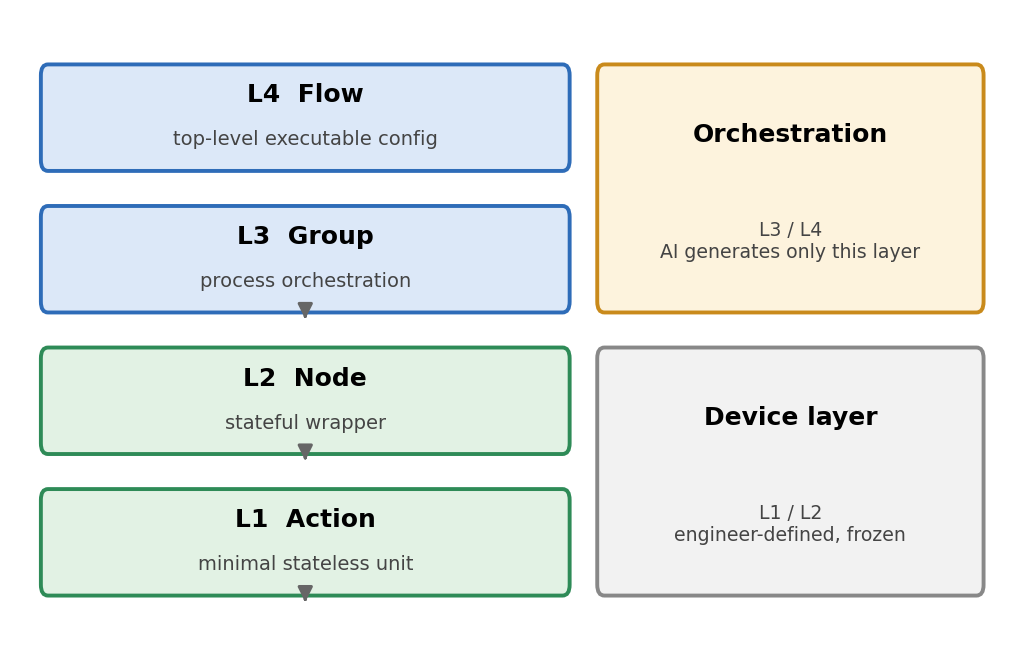
\includegraphics[width=\columnwidth]{fig1_four_layer.png}
\caption{Four-layer representation and the naming contract.}
\label{fig:layers}
\end{figure}

\textbf{Core schema and composition.} Engineers define L1/L2; AI composes only L3/L4. Each layer is a JSON object. L1 maps declared arguments to an atomic operation's result. L2 references one L1 through \path{action.template}, adding \texttt{params}, an optional \texttt{judge}, timeout/retry settings, and outcome branches. In the beverage benchmark, L2's \texttt{device} binding selects a registry entry containing port and station address; L1 stores only the Modbus protocol data unit (PDU), excluding station address and CRC. L3 requires \texttt{type=group}, \texttt{name}, and \texttt{mode}; its executable bodies contain L2 calls or recursively nested L3 groups, either inline or referenced by \texttt{template}. L4 uses \texttt{type=flow}, \texttt{name}, and a nonempty \texttt{body} of L3 calls, with optional parameter \texttt{profiles}. Thus, orchestration introduces no new device operations.

\textbf{Interfaces and data flow.} The naming contract encodes argument types, return type, and result key, e.g., \path{read_pressure.r_u16_pressure}; the argument segment is omitted for parameter-free calls. Types include signed/unsigned 8-, 16-, and 32-bit integers, float, Boolean, string, hexadecimal string, and array; \texttt{void} denotes no return value. Declarations in \texttt{args} give index, name, type, and optional defaults or constraints. Node \texttt{params} supply positional arguments; group calls bind by declared index or name, falling back to declared defaults. Results are written to the shared variable store under signature keys and optional node-call \texttt{result\_key}; Boolean node results represent judge success. Later steps read them through \texttt{\$\{key\}}. Flow profile values enter the same store. This is shared state, not lexical scope.

\textbf{Control and validity rules.} L3 modes are \texttt{sequence}, \texttt{parallel}, \texttt{loop}, \texttt{if}, and \texttt{switch}. Sequences follow array order; \texttt{if} selects \texttt{then/else}, and \texttt{switch} selects a case or default. Loops specify \texttt{loop.type} and execute \texttt{body}; \texttt{while} tests before the body, \texttt{do-while} after it, and \texttt{count} repeats a specified number of times. Well-formed configurations require resolvable templates, arguments compatible with declarations, and mode-specific fields (e.g., loop conditions and unique case values). These are language requirements, not a claim of complete static type checking. Full field definitions are in \path{docs/manual/}; parsers and execution semantics are in \path{src/} at the revision below.

\textbf{A compact four-layer example.} Listing~\ref{lst:four-layers} follows a clean-in-place (CIP) pressure check from the beverage benchmark at commit \texttt{2e1282f}. L1 decodes a float; L2 checks the 0.3~MPa threshold; L3 selects the pressure sensor. L4 passes flavor and size to \texttt{run\_recipe}, which invokes the CIP group after production. The listing uses aliases \texttt{P} and \texttt{C} for the L1 and L2 bundle-entry paths named in its comments; ellipses omit other fields and steps. A failed judge triggers the archived \texttt{CIP\_PRESSURE\_LOW} error branch.

\begin{lstlisting}[caption={CIP pressure check across L1--L4 (selected fields).},label={lst:four-layers},captionpos=t]
// P: L1_action/all_actions.json/
//    read_fc03_reg0010_le.r_f_value
{"type":"modbus_read_cache","args":[],
 "request":"03 00 10 00 02","parse":{
 "start_byte":2,"length":4,
 "endian":"little","type":"float"}, ...}
// C: L2_node/all_nodes.json/
//    read_fc03_reg0010_le_cip_pressure_low.r_b_check_ok
{"type":"node","action":{"template":"P"},
 "device":"${device}","timeout_ms":3000,
 "judge":{"type":"compare","condition":"ge",
          "value":0.3}, ...}
// L3: step_11_cip_cleaning_sanitizing.group.json
{"type":"group","mode":"sequence", ...,
 "body":[..., {"type":"node","template":"C",
 "device":"PressureSensor","params":[]}, ...]}
// L4: orange_family.json (flavor=0, size=0)
{"type":"flow","name":"orange_family",
 "mode":"sequence","body":[{"type":"group",
 "template":"L3_group/run_recipe.group.json",
 "params":[0,0]}]}
\end{lstlisting}

\subsection{Execution Engine and Safety Mechanisms}

Industrial Config Engine v0.1 (C++17, nlohmann/json, open source) implements the framework:
\begin{itemize}
\item \textbf{L1--L4 data models and loaders:} actions and nodes load from aggregation bundles or single files; cross-layer references resolve through the naming contract.
\item \textbf{Built-in structural validators:} every layer carries \texttt{validate()} checking required fields, body item types, loop type/condition, case uniqueness, node budgets, action/judge/branch forms, parameter declarations, and profile consistency.
\item \textbf{Executor:} runs L3/L4 on a virtual device registry (registers/coils with pluggable behavior models), with a run-time variable store (\texttt{\$\{var\}} resolution), a virtual clock, and an audit log.
\item \textbf{Safety:} (1) AI-generated configurations receive no automatic deployment permission; (2) \path{confirm_between} logs simulated approvals as \path{OPERATOR_CONFIRM}, without waiting for live operator input; (3) execution decisions and state changes are audited; (4) a step budget bounds each run, with typed error classes (\path{REFERENCE_ERROR}, \path{CONDITION_ERROR}, \path{STEP_BUDGET_EXCEEDED}, \texttt{TIMEOUT}).
\end{itemize}

Configurations undergo parsing and structural checks; node/group checks also occur during execution. The simulator traverses parallel bodies sequentially.

\subsection{Three-Gate Verification}

\begin{table}[t]
\caption{Three Verification Gates}
\label{tab:gates}
\centering
\small
\begin{tabular}{|P{1.5cm}|P{1.5cm}|P{2.4cm}|P{1.3cm}|}
\hline
\textbf{Gate} & \textbf{When} & \textbf{Output} & \textbf{Validator}\\
\hline
Structural & load time & pass/fail + error report & engine (auto)\\
\hline
Simulation & pre-deploy & timing trace + typed errors & engine (auto)\\
\hline
Semantic mapping & pre-deploy & NL description + flowchart & human\\
\hline
\end{tabular}
\end{table}

\textbf{Structural validation} parses JSON and applies per-layer checks to required fields, declarations, and composition forms. It is not a complete static type or reference checker: nested templates and references may be checked only when executed. Missing references then yield \path{REFERENCE_ERROR}; some invalid arguments remain accepted (Section~III-C).

\textbf{Simulation execution} runs the configuration on virtual devices with a virtual clock and a step budget, intercepting syntactically invisible errors: undefined variables (\path{CONDITION_ERROR}), non-terminating loops (\path{STEP_BUDGET_EXCEEDED}), and deadline violations (\texttt{TIMEOUT}). Detection during simulation does not imply that no preceding simulated write occurred.

\textbf{Semantic mapping} reverse-translates a configuration into natural language and a flowchart so a process engineer can compare it against the original requirement---the gate that checks \emph{intent}, using semantic consistency rather than structural match as the correctness criterion~\cite{agents4plc}. Fig.~\ref{fig:gates} shows the pipeline.

\textbf{Independent-review protocol.} The companion artifact supplies 26 blinded candidates: eight distinct normal controls and 18 mutants. Each packet includes requirements, configuration, invocation, and supporting definitions; reference labels and repairs are withheld. Two reviewers independently record accept/reject, a reason, and review time before seeing the key; the second must not have participated in generation or repair. The scorer requires complete responses and reports raw agreement, Cohen's $\kappa$, disagreements, and errors against the reference labels. These materials make the proposed reliability test reproducible; independent human responses have not yet been collected, so no agreement result is claimed.

\begin{figure}[t]
\centering
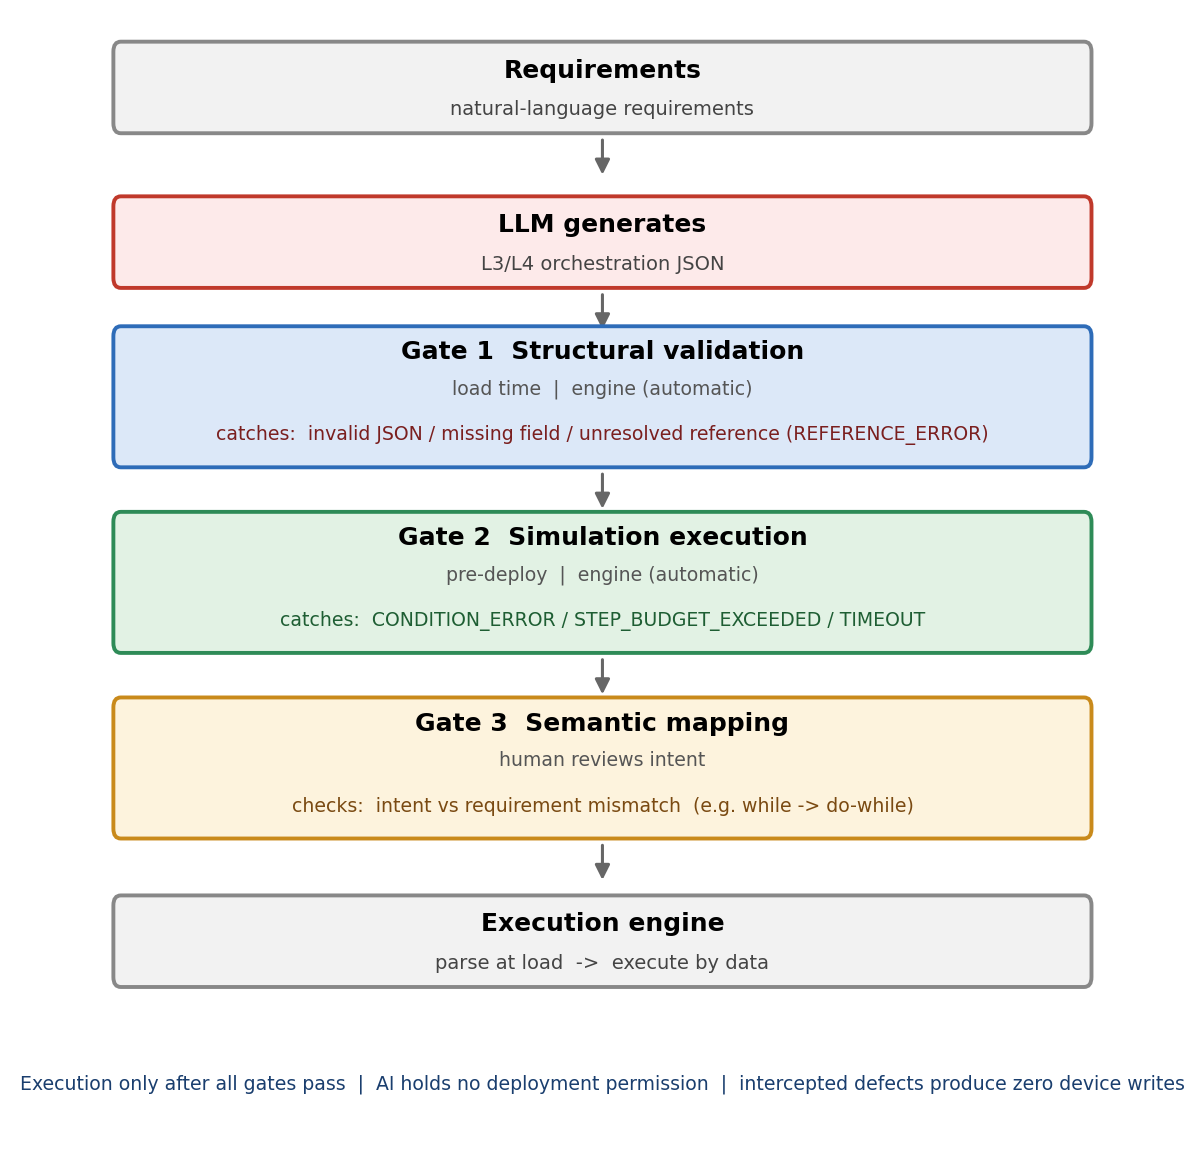
\includegraphics[width=\columnwidth]{fig2_three_gates.png}
\caption{Workflow schematic; references may be checked at run time. The zero-write annotation concerns only the three original injections.}
\label{fig:gates}
\end{figure}

\section{Experiments and Evaluation}

\subsection{Experimental Setup}

We prompted DeepSeek V4-Flash with device manuals (L1/L2 capability lists) and requirements to generate L3/L4 configurations, then passed the outputs through the three gates. The log in \path{examples/docs/experiment_log.md} summarizes the cases and points to archived requirements and drafts (Table~\ref{tab:cases}). The separately constructed beverage benchmark in \path{examples/beverage_full/} evaluates representation size, reuse, and simulated trace agreement (Section~IV), not LLM generation success.

\begin{table}[t]
\caption{Test Cases (as archived in the repository)}
\label{tab:cases}
\centering
\small
\begin{tabular}{|c|P{1.6cm}|c|c|c|c|c|}
\hline
\textbf{Case} & \textbf{Name} & \textbf{Dev.} & \textbf{L1} & \textbf{L2} & \textbf{L3} & \textbf{L4}\\
\hline
T1 & vacuum control & 3 & 11 & 10 & 7 & 1\\
\hline
T2 & motor feeding & 4 & 18 & 22 & 12 & 1\\
\hline
T3 & leak testing & 3 & 26 & 30 & 10$^{*}$ & 1\\
\hline
\end{tabular}
\\[2pt]
{\footnotesize $^{*}$T3 reuses three positioning groups and their L1/L2 layers from T2 (cross-line reuse).}
\end{table}

\subsection{Error-Space Compression and Cross-Line Reuse}

Table~\ref{tab:size} counts the three configurations as archived. Taking T2: the archived 537-line orchestration JSON uses 30 distinct reference names; unresolved names are rejected during reference checking, while the device-driver layer (18 actions, 22 nodes, 1085 lines) is not modified by the LLM. This restricts generated artifacts to compositions of available capabilities, excluding edits to frozen register operations. Bad references, types, sequencing, and parameter choices can still cause errors. The vocabulary counts describe reference usage, not a measured reduction in error probability.

Cross-line reuse: 3 of T3's 10 L3 groups (\path{precise_positioning}, \path{run_pr_with_wait}, \path{jog_find_sensor}) are taken directly from T2's library---30\% of T3's group definitions---with the L1/L2 layer brought in whole. Reuse is reference-by-name with compatible supporting layers, making verified process knowledge a portable, searchable data asset; new hardware may still require mapping adaptation.

\begin{table}[t]
\caption{Configuration Size and Controlled Vocabulary}
\label{tab:size}
\centering
\small
\begin{tabular}{|c|P{2.7cm}|P{2.7cm}|c|}
\hline
\textbf{Case} & \textbf{L3/L4 (LLM)} & \textbf{L1/L2 (frozen)} & \textbf{Vocab}\\
\hline
T1 & 8 files / 424 lines & 8 files / 445 lines & 16\\
\hline
T2 & 13 files / 537 lines & 14 files / 1085 lines & 30\\
\hline
T3 & 11 files / 818 lines & 19 files / 2175 lines & 45\\
\hline
\end{tabular}
\end{table}

\subsection{Defect Detection and Repairs}

The three corrected processes complete in simulation: T1 reaches 3~Pa with the pump stopped; T2 saves both feeding positions; T3 reports \path{test_result=PASS} and 79 simulated approval records. These are corrected-case outcomes, not first-attempt generation rates.

\textbf{Controlled configuration mutations.} We apply 18 single-change mutations to eight valid configurations from T1--T3 and the two beverage datasets (Table~\ref{tab:errors}). Some cases exercise individual L3 sub-processes. Each case runs a normal control, a mutant, and an explicit repair restoring the original configuration/invocation: 54 runs in total. The C++ probe separately invokes the top-level parser/validator (S) and the executor (E), which still performs internal structural checks; this is a coverage comparison, not a gate-disabling ablation.

\begin{table}[t]
\caption{Measured Configuration-Defect Outcomes}
\label{tab:errors}
\centering
\small
\setlength{\tabcolsep}{4pt}
\begin{tabular}{|P{4.45cm}|r|r|r|r|}
\hline
\textbf{Mutation class} & \textbf{N} & \textbf{S} & \textbf{E} & \textbf{O}\\
\hline
Invalid outer item / missing condition & 2 & 2 & 2 & 0\\
\hline
Undefined variable / endless loop & 2 & 0 & 2 & 0\\
\hline
Invalid nested loop schema & 1 & 0 & 1 & 0\\
\hline
Missing node / unregistered device & 3 & 0 & 3 & 0\\
\hline
Unavailable recipe / wrong sensor & 2 & 0 & 2 & 0\\
\hline
Missing / wrong-type / out-of-range PR argument & 3 & 0 & 0 & 3\\
\hline
Wrong predicate / reported result & 2 & 0 & 0 & 2\\
\hline
Short CIP wait / reordered step / omitted check & 3 & 0 & 0 & 3\\
\hline
\textbf{Total} & \textbf{18} & \textbf{2} & \textbf{10} & \textbf{8}\\
\hline
\end{tabular}
\\[2pt]
{\footnotesize N: mutations; S: top-level structural rejection; E: execution-path rejection, including S; O: accepted by both but distinguished by an external regression oracle.}
\end{table}

The execution path rejects 10/18 mutants (55.6\%), eight beyond the top-level structural checks. Rejections include \path{CONDITION_ERROR}, \path{REFERENCE_ERROR}, \texttt{TIMEOUT}, and structural/range failures. No normal run is rejected (0/18 runs, eight distinct controls). All 18 repairs reproduce their controls. The remaining eight mutants finish with \texttt{SUCCESS}: missing, nonnumeric, or oversized PR arguments; a reversed leak predicate or wrong result; and shortened CIP time, reordered operations, or an omitted level check. Thus, typed names and successful execution alone do not establish valid parameters or correct process intent.

The external oracle compares timed \texttt{ROUTE}/\texttt{CHANGE} events, final variables, and virtual device state with a known-good run; it distinguishes all eight accepted mutants. It is neither an engine gate nor independent human review, and exact trace matching is a regression criterion rather than a general equivalence proof. Mutations are hand-selected; this sample's rejection proportion is not a detection rate for naturally generated LLM errors. Repairs are explicit restorations, not automatically inferred fixes.

\textbf{A traced T2 correction.} The archived intermediate draft describes the task as \emph{start PR motion, then poll until motion completes} (translated); it is not a complete original prompt/first-response transcript. Manual schema review identifies unsupported \texttt{while}/\texttt{break\_if} body items and \texttt{steps} instead of \texttt{body}. Listing~\ref{lst:correction} shows the draft fragment and corrected polling body from \path{examples/example2/}; the full draft is in \path{examples/docs/sample2_feeding/1.txt}. The repaired group reads \texttt{motion\_done}, waits 100~ms, then tests completion. The draft already read status before its break. This is a schema-repair illustration, separate from the automatic mutation experiment; it does not establish identical timing or that this draft used an undefined completion variable.

\begin{lstlisting}[float=t,caption={T2 polling: archived fragment and repaired group.},label={lst:correction},captionpos=t]
// Archived intermediate draft (selected fields)
"type":"while",
"steps":[..., {"type":"break_if","condition":{
 "type":"expression",
 "expression":"${motion_done} == true"}}, ...]
// Repaired polling group
{"type":"group","name":"Loop wait motion done",
 "mode":"loop","timeout_ms":"${timeout}",
 "loop":{"type":"do-while",
         "condition":"${motion_done} != true"},
 "body":[
  {"type":"node","template":
   "L2_node/leadshine_nodes.json/check_motion_done.r_b_motion_done",
   "params":[]},
  {"type":"node","template":
   "L2_node/wait_nodes.json/wait_ms.u16.r_b_wait_done",
   "params":[100]}]}
\end{lstlisting}

\subsection{Configuration Time}

\begin{table}[t]
\caption{Configuration and Verification Time}
\label{tab:time}
\centering
\small
\begin{tabular}{|P{3.0cm}|c|c|c|}
\hline
\textbf{Stage} & \textbf{T1} & \textbf{T2} & \textbf{T3}\\
\hline
LLM initial generation & $\sim$20 s & $\sim$45 s & $\sim$40 s\\
\hline
Structural validation & $<$1 s & $<$1 s & $<$1 s\\
\hline
Simulation execution & $\sim$0.17 s & $\sim$0.04 s & $\sim$0.09 s\\
\hline
Semantic mapping (human) & $\sim$2 min & $\sim$6 min & $\sim$6 min\\
\hline
\end{tabular}
\end{table}

The rows involve different actors and objects: the LLM generates the configuration text (T1: 424 lines, $\sim$20~s); validation and simulation are automatic (the simulator runs 923 atomic actions over 88.5 virtual seconds to converge T1's pump-down, in 0.17~s); semantic mapping is a human review of the 424-line structure, not the 923 actions. These stage records assume existing device libraries and simulation models; total development and repair effort is not measured. Human review is the bottleneck ($>$85\% of T3's reported stage time), consistent with studies treating it as the key cost metric for LLM-assisted control engineering~\cite{agents4plc}.

\section{Discussion}

\subsection{Key Findings}

\textbf{Layered isolation restricts the generated surface.} The T2 counts (Table~\ref{tab:size}) illustrate fixed device implementations and composable interfaces, without guaranteeing all permitted compositions.

\textbf{Measured checks have distinct limits.} Table~\ref{tab:errors} shows eight additional execution-path rejections beyond top-level structural validation, but also eight accepted mutants. Nested schema checking contributes to this increment. The result supports staged checking without isolating each gate's contribution or measuring human-review reliability.

\textbf{Execution exposes dynamic errors.} Undefined loop variables and an always-true pressure loop pass top-level structural checks but produce condition errors or timeouts during execution. This supports testing behavior beyond syntax, as in closed-loop LLM control studies~\cite{wen}; it does not imply rejection before all simulated writes.

\textbf{A configuration corpus begins to form.} The three corrected configurations (29 groups, 3 flows, $\sim$1.8k orchestration lines) form a seed corpus for future process-knowledge mining, with cross-line reuse (Section~III) as its first demonstration.

\textbf{A twelve-stage beverage benchmark.} The baseline combines three flavors with 2~L and 330~mL containers (six recipes); the extension adds 250~mL for all three flavors (nine recipes). Both representations retain loops for two batches of six containers per recipe. The twelve stages are initialization, empty-container feeding, position detection, rinsing, filling positioning, filling, level recheck, capping, coding/labeling, discharge, clean-in-place (CIP), and standby. L4 passes only flavor and size; shared L3 groups select the filling head, recipe duration, and production points. A table maps each production point to precommissioned axis PR points; ordinary moves trigger only changed axes. The library contains 56 L1 actions, 62 L2 nodes, and 20 L3 groups, all exercised by the normal runs.

\textbf{Complete size and extension cost.} Table~\ref{tab:beverage} counts JSON normalized to four-space indentation, UTF-8, unescaped Unicode, and LF endings. Shared definitions are counted once per dataset; both totals include the device registry, and the layered total also includes all point, recipe, and variable tables. Adding 250~mL requires three monolithic files (15,402 lines), versus three L4 files (45 lines) and 183 net data-table lines. One existing L3 constraint also changes the maximum size index from 1 to 2, with no net line increase. The other L1--L3 content and existing recipes remain unchanged. The monolithic form inlines repeated primitives; the layered form shares parameterized definitions, so abstraction levels differ by design. These figures measure configuration size, not developer hours or an isolated layering effect; an equally parameterized non-layered baseline is not evaluated.

\begin{table}[t]
\caption{Complete Beverage Configuration Size (Lines)}
\label{tab:beverage}
\centering
\small
\begin{tabular}{|P{4.4cm}|r|r|}
\hline
\textbf{Component} & \textbf{6 recipes} & \textbf{9 recipes}\\
\hline
Monolithic recipe JSON & 30,804 & 46,206\\
\hline
Shared L1/L2/L3 & 3,931 & 3,931\\
\hline
L4 recipe entries & 90 & 135\\
\hline
Device registry (both schemes) & 89 & 89\\
\hline
Point, recipe, and variable tables & 390 & 573\\
\hline
\textbf{Complete monolithic} & \textbf{30,893} & \textbf{46,295}\\
\hline
\textbf{Complete four-layer} & \textbf{4,500} & \textbf{4,728}\\
\hline
Line reduction & 85.43\% & 89.79\%\\
\hline
\end{tabular}
\end{table}

\textbf{Observed trace equivalence.} Separate Python interpreters execute the saved monolithic and layered configurations against the same deterministic device model. All six baseline and nine extended recipe runs have identical timed traces, comparing port/address, Modbus PDU and response, waits, cache/UI updates, device completion, and product records. Each representation produces 72 and 108 containers, respectively, with 37,122 and 49,020 Modbus exchanges. The original six recipes also retain identical trace hashes after extension. Eleven fault types, including jams, low pressure, insufficient flow, failed level/torque checks, and timeout, are tested on one representative recipe in each dataset (22 cases); both representations report the expected errors with matching traces. These are device/process faults, distinct from the configuration mutations in Section~III-C.

\textbf{Reproducibility.} The engine repository is \url{https://github.com/MingChuQing/industrial_config_engine}. Beverage artifacts are recorded at revision \texttt{2e1282f}; the companion defect suite and this manuscript are archived under tag \path{icdm2026-review-revision-20261003}. From the repository root, \texttt{python}\ \path{scripts/verify_beverage_full.py} regenerates and checks 78 configuration files, reruns the Python simulations and six regression tests, and verifies counts, template coverage, and extension differences. The companion defect suite, \texttt{python}\ \path{scripts/verify_defects.py} (PowerShell: \path{.\verify-defects.ps1}), builds the C++ probe and reruns all 54 control/mutant/repair executions, saving diagnostics and repair diffs under \path{build/defect-verification/}. Generation and review times for T1--T3 remain archived session measurements.

\subsection{Limitations}

Limitations include the human-review bottleneck ($\sim$6 min for T3, $>$85\% of validation time), with graph-based review triage as a future direction~\cite{agents4plc}; a simulation--reality gap (device latency and communication timeouts require hardware-in-the-loop testing)~\cite{safeint}; and a small evaluation scale (three LLM-assisted processes and one constructed beverage benchmark). Both beverage representations derive from common synthetic process plans and share a deterministic device model; trace agreement establishes consistency for tested inputs, not equivalence on arbitrary paths or physical equipment. The mutation matrix and its eight distinct normal controls provide only sample-specific detection and false-rejection evidence. Independent gate ablations, common-task comparisons with other LLM methods, repeated LLM generation trials, performance scaling, and a second engineer's independent accept/reject judgments remain unevaluated. Automatic approval records and regression-oracle checks do not measure the human semantic gate.

\textbf{Threat model.} We assume trusted requirements, L1/L2, and engine code. Malicious requirements, prompt injection, tampering, unauthorized changes, and stale/replayed configurations are unevaluated. Name checks cannot ensure safe parameters or sequencing. Deployment requires separate authorization and plant safety mechanisms; evidence here is simulator-based.

\section{Conclusion and Future Work}

This paper re-conceptualizes industrial process control as a data-driven structured configuration problem and proposes a four-layer framework (L1--L4) with a three-gate verification method. Three contributions stand out: (1) process knowledge represented as structured data, with layered isolation restricting AI participation; (2) the L2 naming contract clarifying the interface across the paradigm gap and enabling cross-line reuse (T3 reuses T2's positioning groups, 30\% of its group definitions); (3) staged verification with measured limits: the execution path rejects 10 of 18 controlled mutants, while eight accepted mutants require a known-good comparison to expose their deviations; independent human-review reliability remains unmeasured. In the synthetic beverage benchmark, complete configurations use 85.43\% fewer lines for six recipes and 89.79\% fewer for nine; extending the shared library requires 228 net lines versus 15,402 for monolithic recipes, with matching traces in the tested simulations.

Future work: (1) hardware-in-the-loop testing and broader evaluation; (2) automated semantic mapping via multi-LLM candidate generation and graph-similarity triage~\cite{agents4plc}; (3) \emph{process-knowledge mining}---building a graph representation of the verified configuration corpus and retrieving similar sub-processes for new lines, turning the framework from a generate--verify system into a mine--reuse system; (4) larger-scale evaluation for generalization; (5) a vendor-published \emph{device SDK} in which manufacturers ship certified L1/L2 definitions together with a pre-packaged L3 template library and per-node natural-language descriptions, so an LLM reads one self-contained SDK and proposes L3/L4 compositions for verification without requiring cross-vendor standardization.

\section*{Acknowledgment}

The initial version of the engine code was written independently by the author; AI-assisted tools (DeepSeek) were used mainly for code normalization, error checking, and debugging assistance, and helped generate test scripts and example configurations. All code and configurations were reviewed, verified, and finalized line by line by the author, who takes full responsibility for the content. The author thanks family members for equipment and time support.

\begin{thebibliography}{6}

\bibitem{iec61131}
IEC 61131-3:2013, \emph{Programmable Controllers --- Part 3: Programming Languages}. Geneva, Switzerland: IEC, 2013.

\bibitem{llm4plc}
M.~Fakih, R.~Dharmaji, Y.~Moghaddas, G.~Quiros, O.~Ogundare, and M.~Al~Faruque, ``LLM4PLC: Harnessing large language models for verifiable programming of PLCs in industrial control systems,'' in \emph{Proc.\ 46th IEEE/ACM Int.\ Conf.\ Softw.\ Eng.: Softw.\ Eng.\ Pract.\ (ICSE-SEIP)}, 2024, pp.~192--203, doi: 10.1145/3639477.3639743.

\bibitem{agents4plc}
Z.~Liu, R.~Zeng, D.~Wang, \emph{et al.}, ``Agents4PLC: Automating closed-loop PLC code generation and verification in industrial control systems using LLM-based agents,'' \emph{arXiv:2410.14209v1}, 2024.

\bibitem{spec2control}
H.~Koziolek, T.~Braun, V.~Ashiwal, S.~Linsbauer, M.~A.~Hansen, and K.~Grotterud, ``Spec2Control: Automating PLC/DCS control-logic engineering from natural language requirements with LLMs --- A Multi-Plant Evaluation,'' in \emph{Proc.\ 48th IEEE/ACM Int.\ Conf.\ Softw.\ Eng.: Softw.\ Eng.\ Pract.\ (ICSE-SEIP)}, 2026, pp.~566--577, doi: 10.1145/3786583.3786897.

\bibitem{safeint}
D.~Schall, ``Safe integration of Large Language Models into industrial process control: a multi-agent architecture with P\&ID-grounded validation,'' \emph{Autonomous Intelligent Systems}, vol.~6, Art. no.~14, 2026, doi: 10.1007/s43684-026-00136-1.

\bibitem{wen}
H.~Wen, J.~Roberts, A.~Zaidi, and A.~McLeod, ``An experiment of using a large language model to control a water tank system,'' \emph{Computers \& Chemical Engineering}, vol.~211, Art. no.~109656, 2026, doi: 10.1016/j.compchemeng.2026.109656.

\end{thebibliography}

\end{document}
